\documentclass[10pt,a4paper]{article}
\usepackage[utf8]{inputenc}
\usepackage{amsmath}
\usepackage{amsfonts}
\usepackage{amssymb}
\usepackage{graphicx}
\graphicspath{ {./images/} }

\title{US Spine Simulation and Results}

\author{Rui Xu \\ MBP rotation\\ Sept 8-Oct 14}

\begin{document}
\maketitle
\newpage

\section{Introduction}

This document will outline my ultrasound code and results. I have constructed a simple two-dimensional simulation using existing code from the k-wave package to construct a two-transistor system.

\section{System 1: Homogeneous Medium, Two Elements, Two Frequencies}

The first system I created was a system of two curved transducers, each with a radius of curvature of 50mm, and each subtending $\pi/2$ radians. The two transducers are driven at frequencies $f_1$ and $f_2$. The focal point of the two transducers are the same. I create the transducers by defining source points at a 50mm radius for $\pi/12 \leq \Theta_1 \leq 5\pi/12$ and $7\pi/12 \leq \Theta_2 \leq 11 \pi/12$. The system setup is shown in the following figure.

\begin{figure}[!h]
\centering
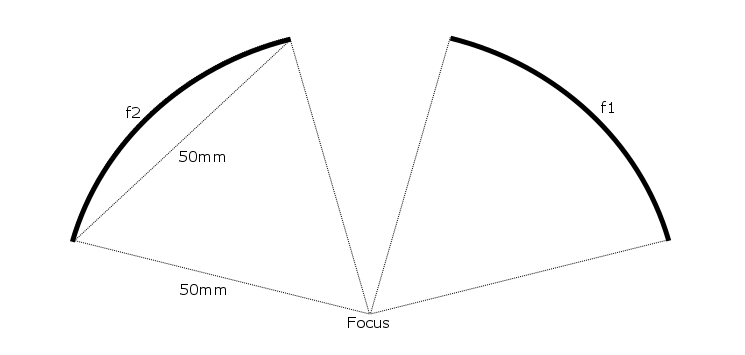
\includegraphics[scale=0.5]{setup1.png}
\centering
\end{figure}

\subsection{Half-Maximum Profiles}

The first test was to vary the frequency $f_1$ of the right hand side transducer, while keeping the frequency of the second transducer constant $f_2 = 0.25$MHz. Implementing multiple frequencies in k-wave require that each source point have its frequency assigned to it. In the current implementation, then I've simply looped over all points, and set the frequency of the source points on the left half of the computational box to $f_2$ and those on the right half to $f_1$. Take care with the current code if you move the transducers around. It may be advisable to write a foolproof version of the frequency assignment part of the code.\\

We are interested in the pressure profile of the system near the focal point, for different frequencies $0.15 \text{MHz} \leq f_1 \leq 0.35 \text{MHz}$, tested in increments of 10kHz. The following figures show the 2D root-mean-square pressure profiles. The points of half-maximum pressure are outlined in black.

\begin{figure}[!h]
\hspace*{-5cm}                                                    
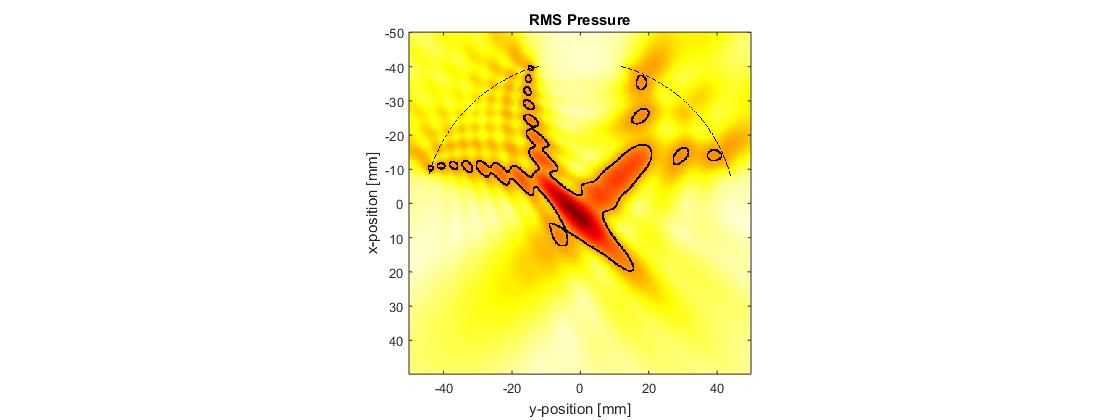
\includegraphics[scale=0.6]{f150kHz}
\caption{RMS pressure profile for $f_1 = 0.15$MHz, $f_2 = 0.25$MHz}
\end{figure}
\begin{figure}[!h]
\hspace*{-5cm}                                                    
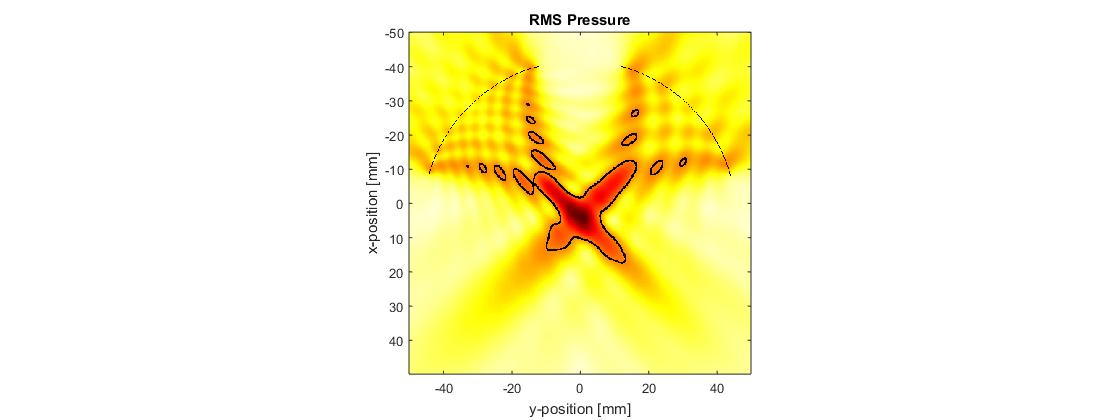
\includegraphics[scale=0.6]{f160kHz}
\caption{RMS pressure profile for $f_1 = 0.16$MHz, $f_2 = 0.25$MHz}
\end{figure}
\begin{figure}[!h]
\hspace*{-5cm}                                                    
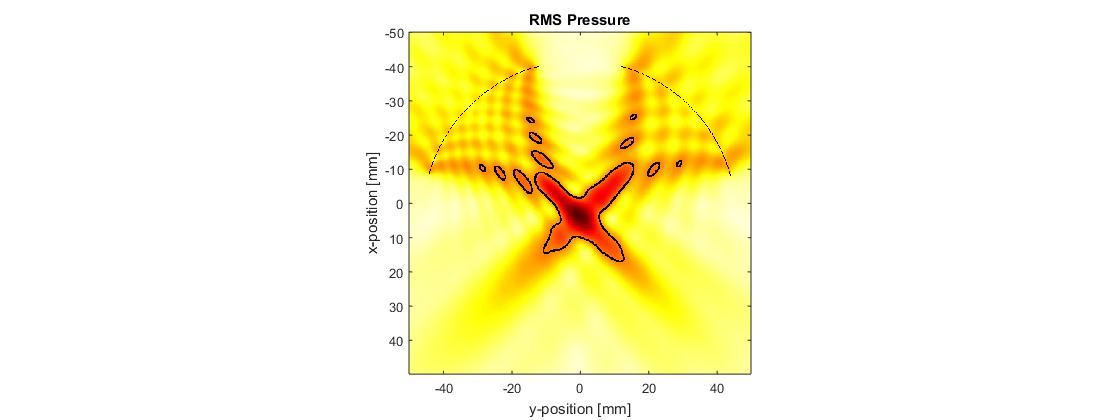
\includegraphics[scale=0.6]{f170kHz}
\caption{RMS pressure profile for $f_1 = 0.17$MHz, $f_2 = 0.25$MHz}
\end{figure}
\begin{figure}[!h]
\hspace*{-5cm}                                                    
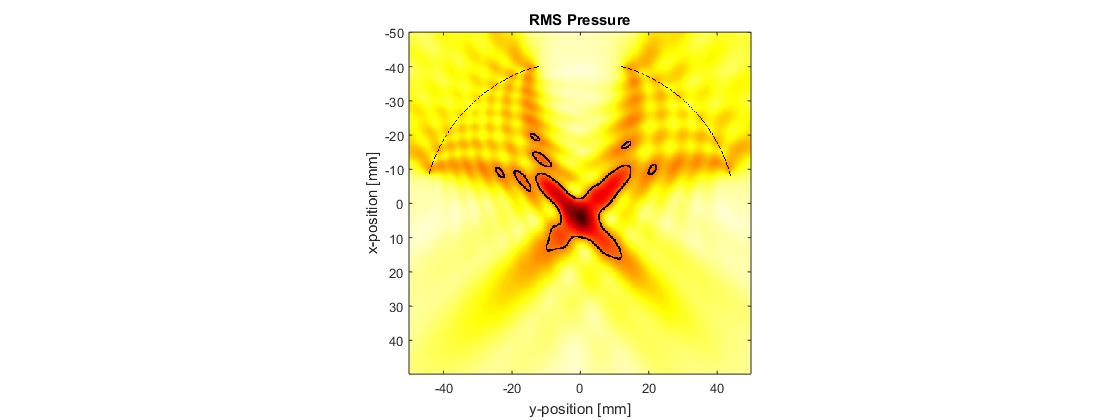
\includegraphics[scale=0.6]{f180kHz}
\caption{RMS pressure profile for $f_1 = 0.18$MHz, $f_2 = 0.25$MHz}
\end{figure}
\begin{figure}[!h]
\hspace*{-5cm}                                                    
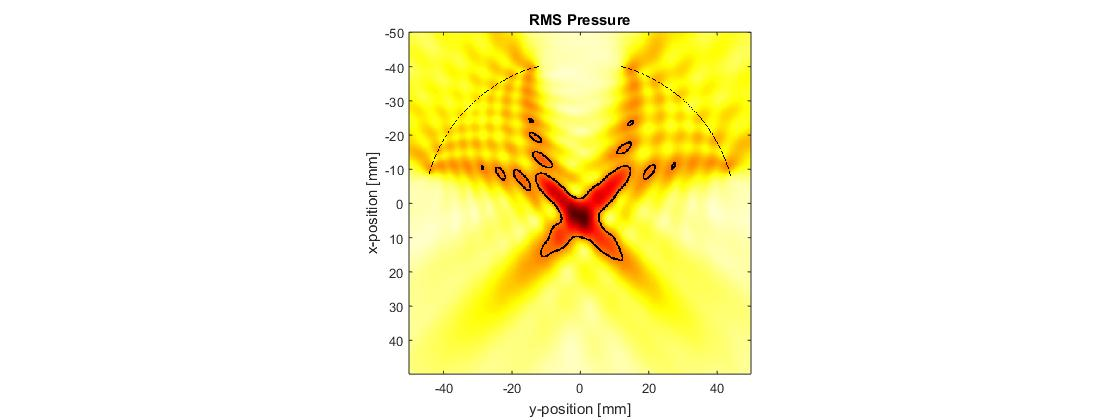
\includegraphics[scale=0.6]{f190kHz}
\caption{RMS pressure profile for $f_1 = 0.19$MHz, $f_2 = 0.25$MHz}
\end{figure}
\begin{figure}[!h]
\hspace*{-5cm}                                                    
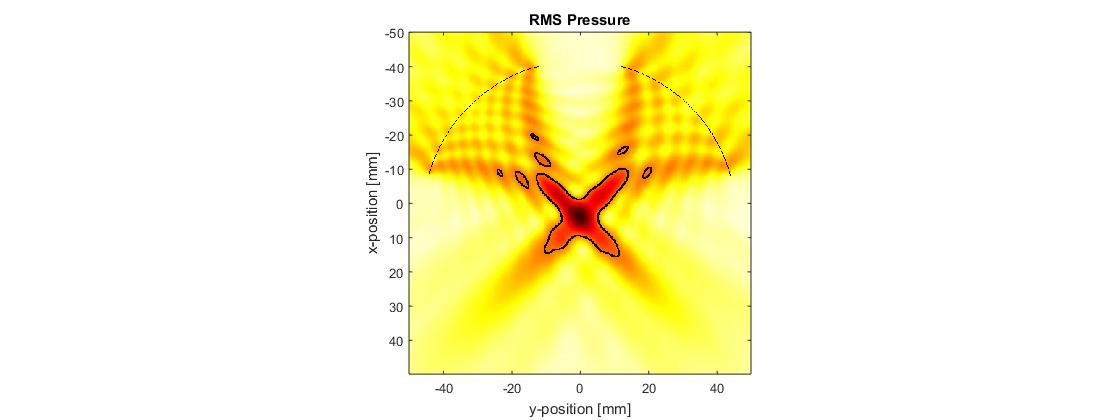
\includegraphics[scale=0.6]{f200kHz}
\caption{RMS pressure profile for $f_1 = 0.20$MHz, $f_2 = 0.25$MHz}
\end{figure}
\begin{figure}[!h]
\hspace*{-5cm}                                                    
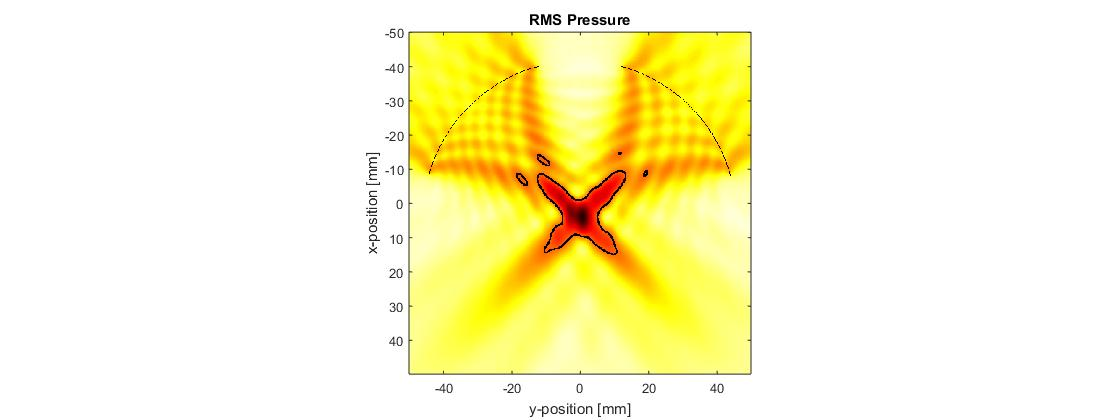
\includegraphics[scale=0.6]{f210kHz}
\caption{RMS pressure profile for $f_1 = 0.21$MHz, $f_2 = 0.25$MHz}
\end{figure}
\begin{figure}[!h]
\hspace*{-5cm}                                                    
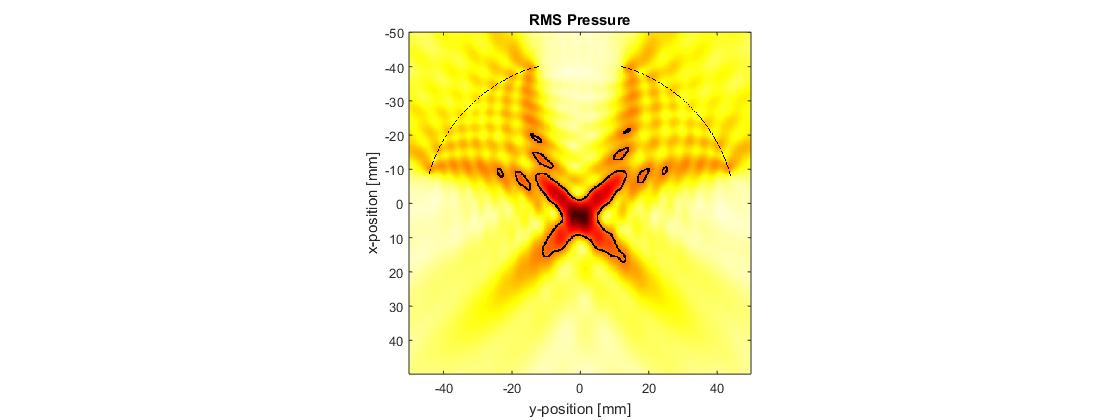
\includegraphics[scale=0.6]{f220kHz}
\caption{RMS pressure profile for $f_1 = 0.22$MHz, $f_2 = 0.25$MHz}
\end{figure}
\begin{figure}[!h]
\hspace*{-5cm}                                                    
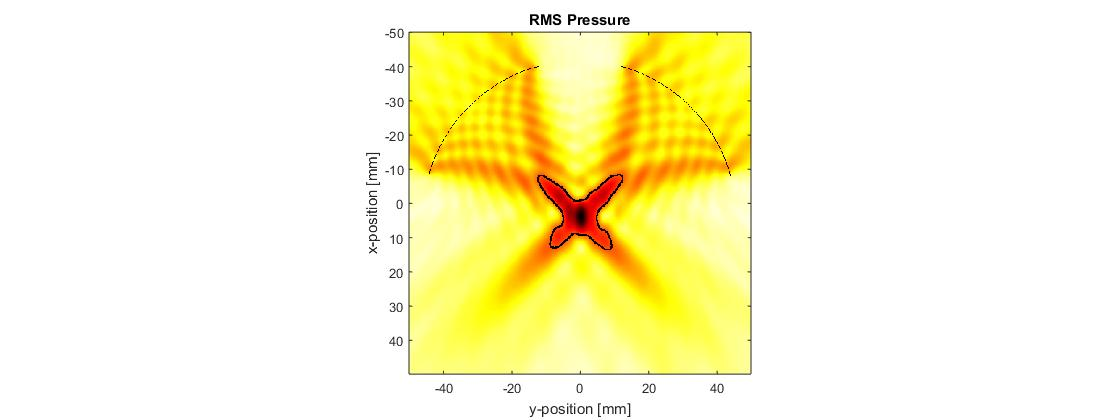
\includegraphics[scale=0.6]{f230kHz}
\caption{RMS pressure profile for $f_1 = 0.23$MHz, $f_2 = 0.25$MHz}
\end{figure}
\begin{figure}[!h]
\hspace*{-5cm}                                                    
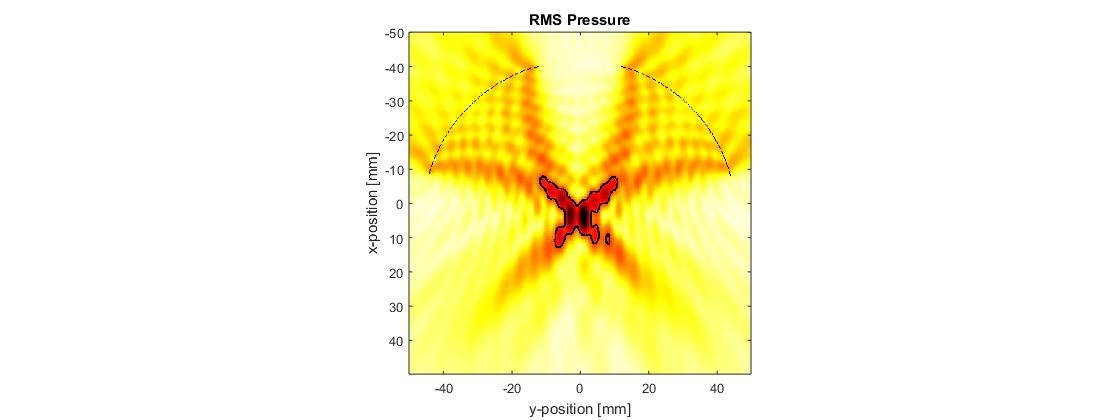
\includegraphics[scale=0.6]{f240kHz}
\caption{RMS pressure profile for $f_1 = 0.24$MHz, $f_2 = 0.25$MHz}
\end{figure}
\begin{figure}[!h]
\hspace*{-5cm}                                                    
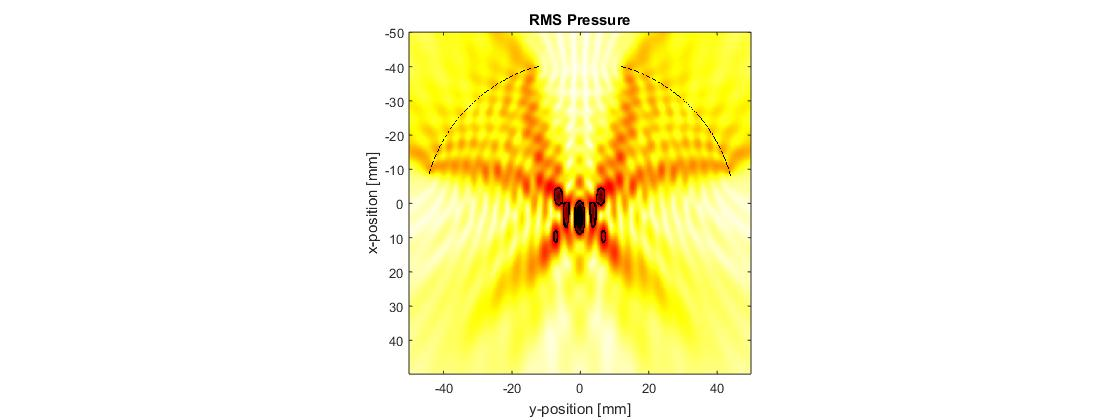
\includegraphics[scale=0.6]{f250kHz}
\caption{RMS pressure profile for $f_1 = 0.25$MHz, $f_2 = 0.25$MHz}
\end{figure}
\begin{figure}[!h]
\hspace*{-5cm}                                                    
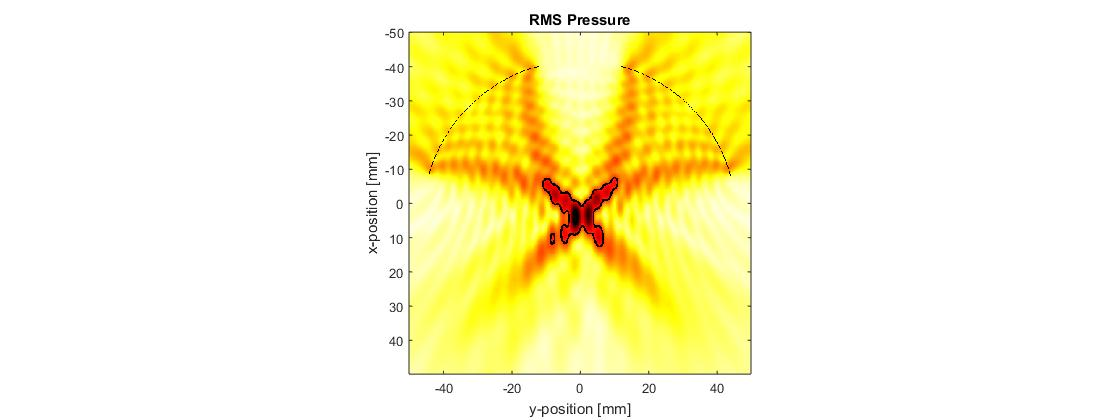
\includegraphics[scale=0.6]{f260kHz}
\caption{RMS pressure profile for $f_1 = 0.26$MHz, $f_2 = 0.25$MHz}
\end{figure}
\begin{figure}[!h]
\hspace*{-5cm}                                                    
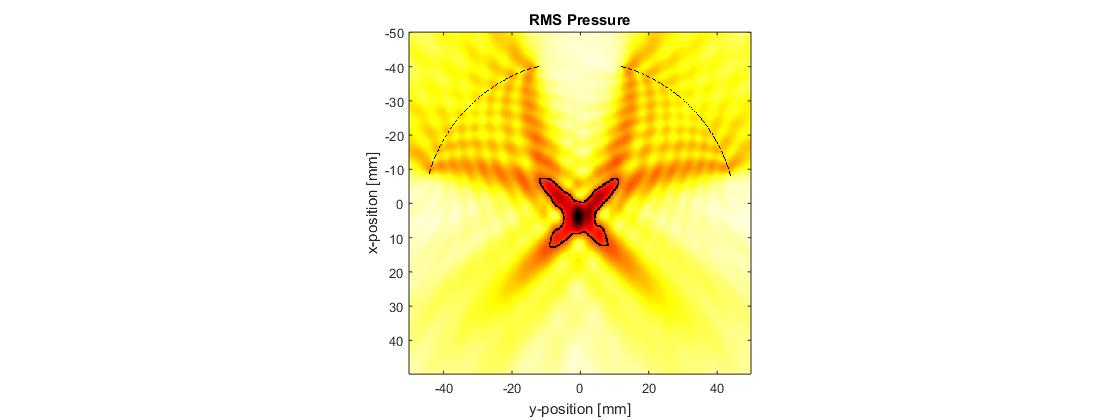
\includegraphics[scale=0.6]{f270kHz}
\caption{RMS pressure profile for $f_1 = 0.27$MHz, $f_2 = 0.25$MHz}
\end{figure}
\begin{figure}[!h]
\hspace*{-5cm}                                                    
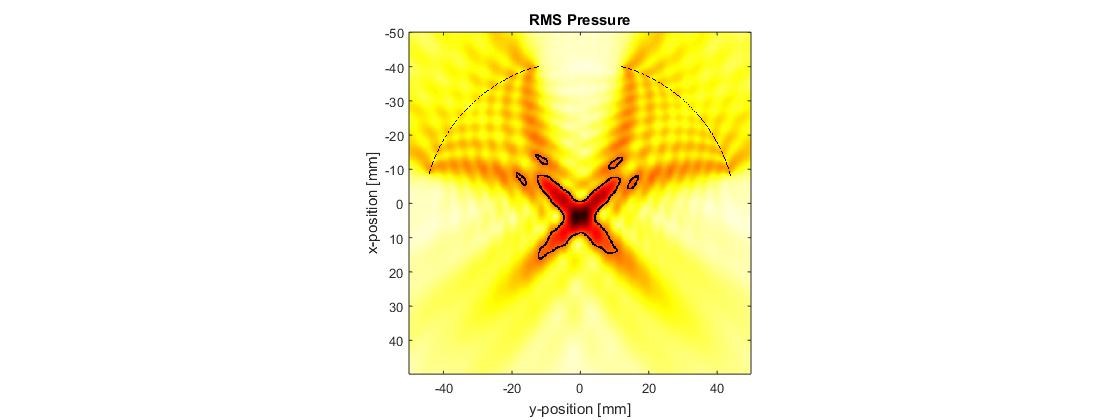
\includegraphics[scale=0.6]{f280kHz}
\caption{RMS pressure profile for $f_1 = 0.28$MHz, $f_2 = 0.25$MHz}
\end{figure}
\begin{figure}[!h]
\hspace*{-5cm}                                                    
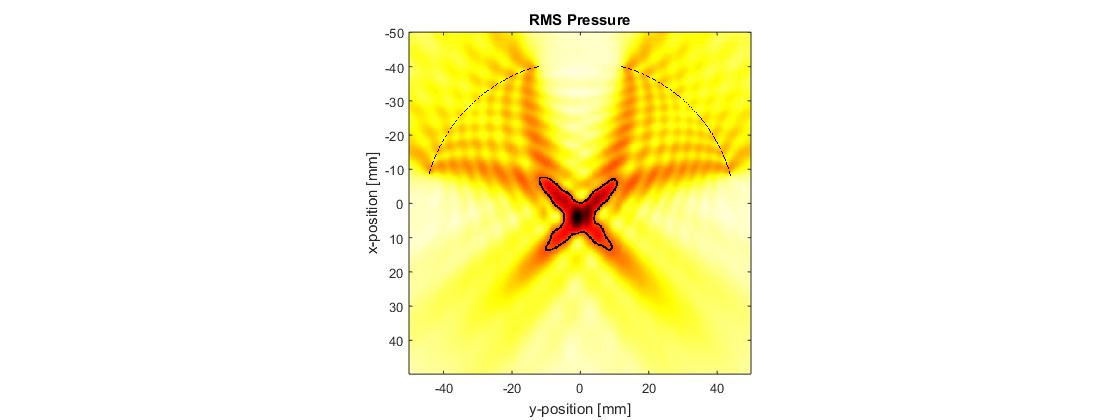
\includegraphics[scale=0.6]{f290kHz}
\caption{RMS pressure profile for $f_1 = 0.29$MHz, $f_2 = 0.25$MHz}
\end{figure}
\begin{figure}[!h]
\hspace*{-5cm}                                                    
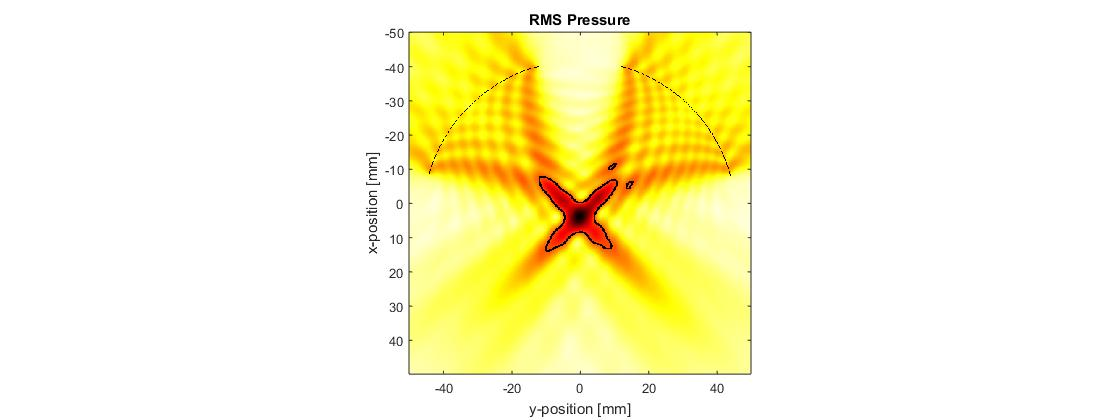
\includegraphics[scale=0.6]{f300kHz}
\caption{RMS pressure profile for $f_1 = 0.30$MHz, $f_2 = 0.25$MHz}
\end{figure}
\begin{figure}[!h]
\hspace*{-5cm}                                                    
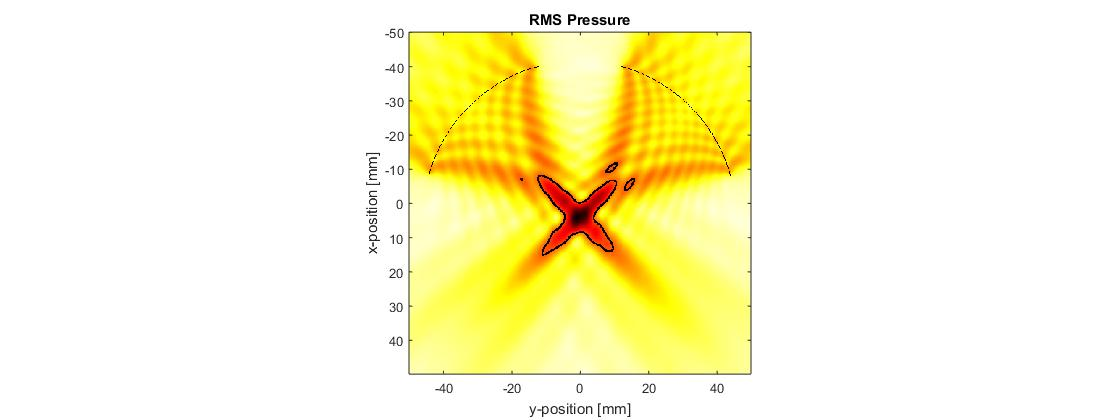
\includegraphics[scale=0.6]{f310kHz}
\caption{RMS pressure profile for $f_1 = 0.31$MHz, $f_2 = 0.25$MHz}
\end{figure}
\begin{figure}[!h]
\hspace*{-5cm}                                                    
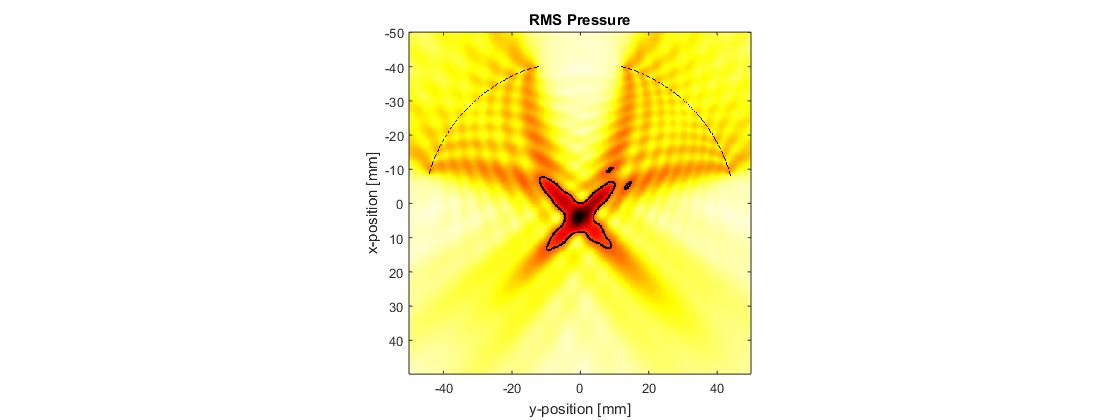
\includegraphics[scale=0.6]{f320kHz}
\caption{RMS pressure profile for $f_1 = 0.32$MHz, $f_2 = 0.25$MHz}
\end{figure}
\begin{figure}[!h]
\hspace*{-5cm}                                                    
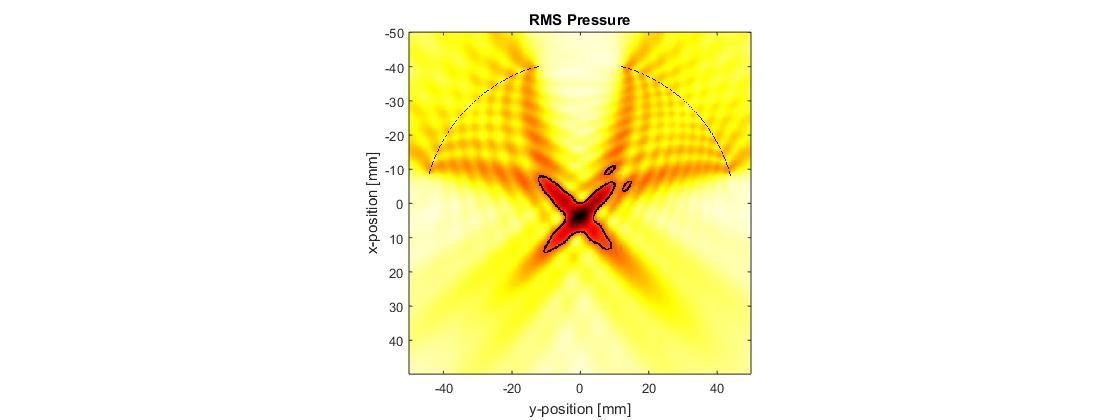
\includegraphics[scale=0.6]{f330kHz}
\caption{RMS pressure profile for $f_1 = 0.33$MHz, $f_2 = 0.25$MHz}
\end{figure}
\begin{figure}[!h]
\hspace*{-5cm}                                                    
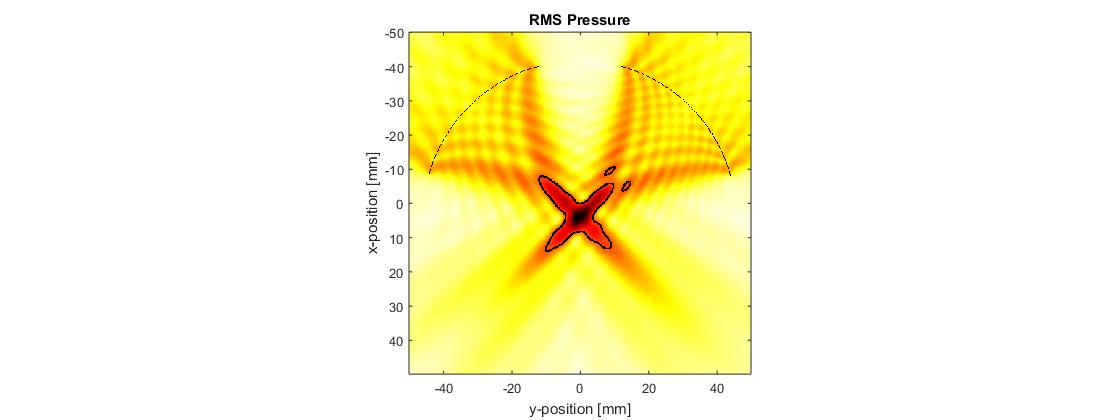
\includegraphics[scale=0.6]{f340kHz}
\caption{RMS pressure profile for $f_1 = 0.34$MHz, $f_2 = 0.25$MHz}
\end{figure}
\begin{figure}[!h]
\hspace*{-5cm}                                                    
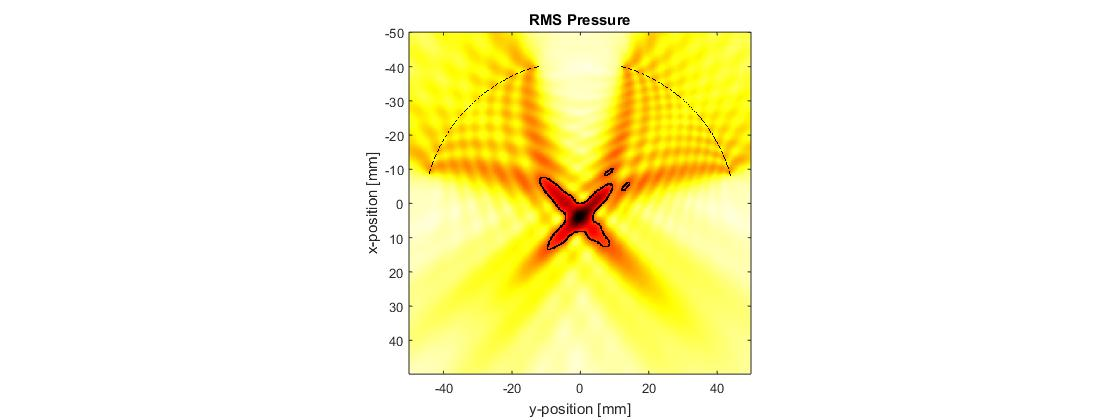
\includegraphics[scale=0.6]{f350kHz}
\caption{RMS pressure profile for $f_1 = 0.35$MHz, $f_2 = 0.25$MHz}
\end{figure}
\newpage

 \subsection{FWHM for different frequencies}

Another informative metric can be the FWHM of the profile. However, this is more useful for pressure profiles that are approximately Gaussian. The method I used for finding the points with half maximum pressure returns coordinates for all points, not just those around the central maximum. This is remediable, but the profiles remain non-circulate. The FWHM of the distributions can easily be calculated from the coordinates ($x_{HM},y_{HM}$) by first calculating the coordinate of the centre of the HM points ($x_{HMc}, y_{HMc})$:
\begin{equation}
x_{HMc} = \frac{1}{N} \sum_{i=1}^N x_{HM_i} \cdot dx, \quad \quad x_{HMc} = \frac{1}{N} \sum_{i=1}^N x_{HM_i} \cdot dx
\end{equation}
where $N$ is the number of HM points. We can calculate the average distance $d$ of the HM points from the HM centre using:
\begin{equation}
d = \frac{1}{N}  \sum_{i=1}^N \sqrt{ (x_{HM_i} - x_{HMc})^2 + (y_{HM_i} - y_{HMc})^2} \cdot dx
\end{equation}
The FWHM is then approximately equal to two times the average distance between an HM point and the centre of the HM point distribution. For HM distributions that are highly non-Gaussian, then there is little purpose in calling it the FWHM - it's simply the average width of the half-maximum RMS pressure profile. Despite this, I'll continue calling it FWHM for the time being. The FWHM is shown for 200kHz$\leq f_1 \leq$ 300kHz in Figure \ref{FWHM_freq}.

\begin{figure}[!h]\label{FWHM_freq}
\centering
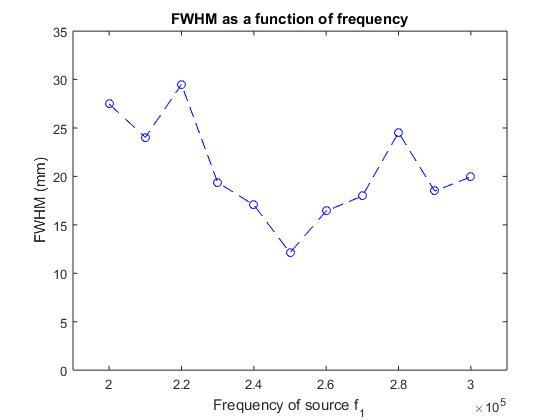
\includegraphics[scale=0.6]{FWHM_freq}
\caption{The FWHM of the RMS pressure distribution for 200kHz$\leq f_1 \leq$ 300kHz, $f_2 = 250$kHz.}
\end{figure}


\subsection{Centre of HM profile}

I've included this for curiosity's sake. Here I plot the centre of the FWHM profile, for 200kHz$\leq f_1 \leq$ 300kHz.
\begin{figure}[!h]
\centering
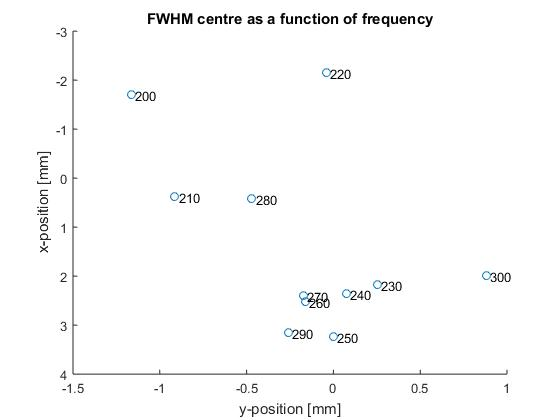
\includegraphics[scale=0.6]{FWHM_centre}
\caption{The coordinates of the centre of the FWHM profile of the RMS pressure distribution for 200kHz$\leq f_1 \leq$ 300kHz, $f_2 = 250$kHz.}
\end{figure}

\subsection{Maximum RMS Pressure}

We are also interested in the location of the maximum RMS intensity for different frequencies. These are shown in the following Figure \ref{RMS_Max}. 

\begin{figure}[!h] \label{RMS_Max}
\centering
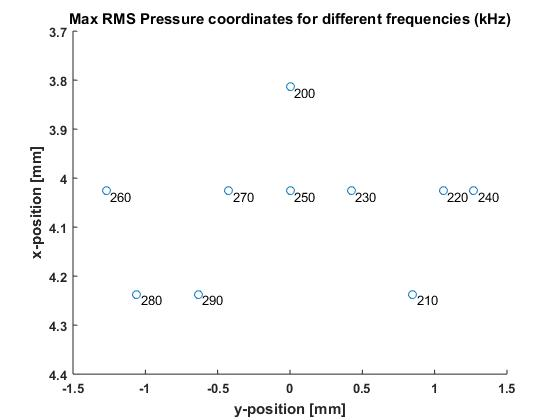
\includegraphics[scale=0.65]{Max_RMS_pressure_coords}
\caption{The Maximum RMS pressure location for 200kHz$\leq f_1 \leq$300kHz.} 
\end{figure}

There does not appear to be any pattern in the location of the maximum RMS pressure coordinates. In the x-dimension, the maxima are confined to within three computational grid points, approximately +4mm away from the focal point of the independent transducers. In the y-dimension, the maxima remain closely clustered around the focal point. Generally, the maximum RMS pressure is much more highly clustered than the FWHM centre.

\section{Adding Inclusions to the Simulation}

The next step to increasing the complexity of the simulation is to add an inclusion near the focal point of the two transducers. The acoustic properties that k-wave includes are the sound speed within the medium, the ambient density distribution within the medium, a nonlinearity parameter, the power law absorption prefactor $\alpha_0$, and the power law absorption exponent $y$, where the power law is:
\begin{equation}
\alpha(f) = \alpha_0 \omega^y, 	\quad \omega = 2 \pi f 
\end{equation}

The simulation package, k-wave, doesn't include all non-linear effects, but does include two additional non-linear terms to attempt to account for all non-linear behaviour. These terms are defined as BonA in k-wave, where A and B are the first and second terms in the Taylor series expansion of the relation between the materials pressure and density.

All of these variables can be set as spatially heterogeneous in k-wave. In order to make an accurate simulation, I will need the acoustic properties of the medium I'll be simulating - namely water, bone, fat, nerve tissue, etc. Some of these are available in "Physical Properties of Tissue", a reference book by Francis A. Duck, and referenced by Chris Diederich in his interstitial spine simulation work.



\subsection{Results from Cadavers}

\subsection{Acoustic Properties}

\subsection{Simulation}

\end{document}